\documentclass{standalone}
\usepackage{tikz}
\usetikzlibrary{patterns, positioning}


\begin{document}
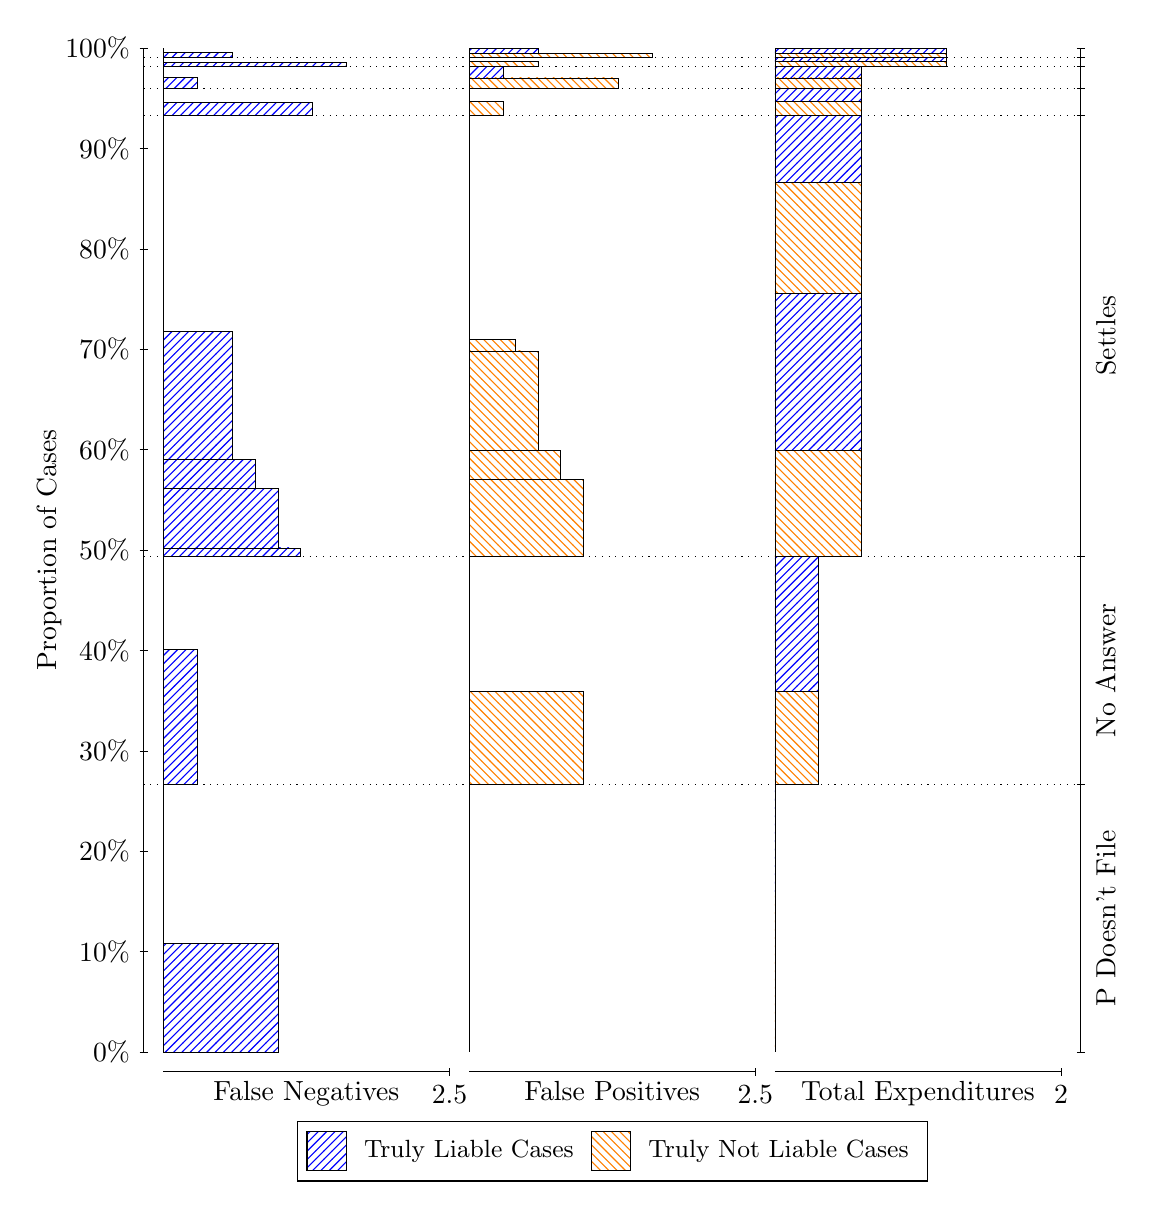
\begin{tikzpicture}
\draw[black, very thin] (1.5,1.75) -- (1.5,14.5);
\node[rotate=90, text=black, anchor=center] at (0.3, 8.125) {Proportion of Cases};
\draw[black, very thin] (1.45,1.75) -- (1.55,1.75);
\node[text=black, anchor=east] at (1.45, 1.75) {0\%};
\draw[black, very thin] (1.45,3.025) -- (1.55,3.025);
\node[text=black, anchor=east] at (1.45, 3.025) {10\%};
\draw[black, very thin] (1.45,4.3) -- (1.55,4.3);
\node[text=black, anchor=east] at (1.45, 4.3) {20\%};
\draw[black, very thin] (1.45,5.575) -- (1.55,5.575);
\node[text=black, anchor=east] at (1.45, 5.575) {30\%};
\draw[black, very thin] (1.45,6.85) -- (1.55,6.85);
\node[text=black, anchor=east] at (1.45, 6.85) {40\%};
\draw[black, very thin] (1.45,8.125) -- (1.55,8.125);
\node[text=black, anchor=east] at (1.45, 8.125) {50\%};
\draw[black, very thin] (1.45,9.4) -- (1.55,9.4);
\node[text=black, anchor=east] at (1.45, 9.4) {60\%};
\draw[black, very thin] (1.45,10.675) -- (1.55,10.675);
\node[text=black, anchor=east] at (1.45, 10.675) {70\%};
\draw[black, very thin] (1.45,11.95) -- (1.55,11.95);
\node[text=black, anchor=east] at (1.45, 11.95) {80\%};
\draw[black, very thin] (1.45,13.225) -- (1.55,13.225);
\node[text=black, anchor=east] at (1.45, 13.225) {90\%};
\draw[black, very thin] (1.45,14.5) -- (1.55,14.5);
\node[text=black, anchor=east] at (1.45, 14.5) {100\%};

\draw[black, very thin] (13.4,1.75) -- (13.4,14.5);
\draw[black, very thin] (13.35,1.75) -- (13.45,1.75);
\node[anchor=west] at (13.35, 1.75) {};
\draw[black, very thin] (13.35,5.1439) -- (13.45,5.1439);
\node[anchor=west] at (13.35, 5.1439) {};
\draw[black, very thin] (13.35,8.0479) -- (13.45,8.0479);
\node[anchor=west] at (13.35, 8.0479) {};
\draw[black, very thin] (13.35,13.647) -- (13.45,13.647);
\node[anchor=west] at (13.35, 13.647) {};
\draw[black, very thin] (13.35,13.984) -- (13.45,13.984);
\node[anchor=west] at (13.35, 13.984) {};
\draw[black, very thin] (13.35,14.269) -- (13.45,14.269);
\node[anchor=west] at (13.35, 14.269) {};
\draw[black, very thin] (13.35,14.383) -- (13.45,14.383);
\node[anchor=west] at (13.35, 14.383) {};
\draw[black, very thin] (13.35,14.5) -- (13.45,14.5);
\node[anchor=west] at (13.35, 14.5) {};

\draw[black, very thin, pattern color=blue, pattern=north east lines] (1.75,1.75) rectangle (3.2033,3.128);
\draw[black, very thin, pattern color=orange, pattern=north west lines] (1.75,3.128) rectangle (1.75,5.1439);
\draw[black, very thin, pattern color=blue, pattern=north east lines] (1.75,5.1439) rectangle (2.186,6.8666);
\draw[black, very thin, pattern color=orange, pattern=north west lines] (1.75,6.8666) rectangle (1.75,8.0479);
\draw[black, very thin, pattern color=blue, pattern=north east lines] (1.75,8.0479) rectangle (3.494,8.1487);
\draw[black, very thin, pattern color=blue, pattern=north east lines] (1.75,8.1487) rectangle (3.3487,8.1518);
\draw[black, very thin, pattern color=blue, pattern=north east lines] (1.75,8.1518) rectangle (3.2033,8.9049);
\draw[black, very thin, pattern color=blue, pattern=north east lines] (1.75,8.9049) rectangle (2.9127,9.2749);
\draw[black, very thin, pattern color=blue, pattern=north east lines] (1.75,9.2749) rectangle (2.622,10.9);
\draw[black, very thin, pattern color=orange, pattern=north west lines] (1.75,10.9) rectangle (1.75,13.647);
\draw[black, very thin, pattern color=blue, pattern=north east lines] (1.75,13.647) rectangle (3.6393,13.808);
\draw[black, very thin, pattern color=orange, pattern=north west lines] (1.75,13.808) rectangle (1.75,13.984);
\draw[black, very thin, pattern color=blue, pattern=north east lines] (1.75,13.984) rectangle (2.186,14.13);
\draw[black, very thin, pattern color=orange, pattern=north west lines] (1.75,14.13) rectangle (1.75,14.269);
\draw[black, very thin, pattern color=blue, pattern=north east lines] (1.75,14.269) rectangle (4.0753,14.319);
\draw[black, very thin, pattern color=orange, pattern=north west lines] (1.75,14.319) rectangle (1.75,14.383);
\draw[black, very thin, pattern color=blue, pattern=north east lines] (1.75,14.383) rectangle (2.622,14.448);
\draw[black, very thin, pattern color=orange, pattern=north west lines] (1.75,14.448) rectangle (1.75,14.5);
\draw[black, very thin, pattern color=orange, pattern=north west lines] (5.6333,1.75) rectangle (5.6333,3.766);
\draw[black, very thin, pattern color=blue, pattern=north east lines] (5.6333,3.766) rectangle (5.6333,5.1439);
\draw[black, very thin, pattern color=orange, pattern=north west lines] (5.6333,5.1439) rectangle (7.0867,6.3252);
\draw[black, very thin, pattern color=blue, pattern=north east lines] (5.6333,6.3252) rectangle (5.6333,8.0479);
\draw[black, very thin, pattern color=orange, pattern=north west lines] (5.6333,8.0479) rectangle (7.0867,9.0222);
\draw[black, very thin, pattern color=orange, pattern=north west lines] (5.6333,9.0222) rectangle (6.796,9.3921);
\draw[black, very thin, pattern color=orange, pattern=north west lines] (5.6333,9.3921) rectangle (6.5053,10.65);
\draw[black, very thin, pattern color=orange, pattern=north west lines] (5.6333,10.65) rectangle (6.36,10.654);
\draw[black, very thin, pattern color=orange, pattern=north west lines] (5.6333,10.654) rectangle (6.2147,10.796);
\draw[black, very thin, pattern color=blue, pattern=north east lines] (5.6333,10.796) rectangle (5.6333,13.647);
\draw[black, very thin, pattern color=orange, pattern=north west lines] (5.6333,13.647) rectangle (6.0693,13.824);
\draw[black, very thin, pattern color=blue, pattern=north east lines] (5.6333,13.824) rectangle (5.6333,13.984);
\draw[black, very thin, pattern color=orange, pattern=north west lines] (5.6333,13.984) rectangle (7.5227,14.122);
\draw[black, very thin, pattern color=blue, pattern=north east lines] (5.6333,14.122) rectangle (6.0693,14.269);
\draw[black, very thin, pattern color=orange, pattern=north west lines] (5.6333,14.269) rectangle (6.5053,14.332);
\draw[black, very thin, pattern color=blue, pattern=north east lines] (5.6333,14.332) rectangle (5.6333,14.383);
\draw[black, very thin, pattern color=orange, pattern=north west lines] (5.6333,14.383) rectangle (7.9587,14.435);
\draw[black, very thin, pattern color=blue, pattern=north east lines] (5.6333,14.435) rectangle (6.5053,14.5);
\draw[black, very thin, pattern color=orange, pattern=north west lines] (9.5167,1.75) rectangle (9.5167,3.766);
\draw[black, very thin, pattern color=blue, pattern=north east lines] (9.5167,3.766) rectangle (9.5167,5.1439);
\draw[black, very thin, pattern color=orange, pattern=north west lines] (9.5167,5.1439) rectangle (10.062,6.3252);
\draw[black, very thin, pattern color=blue, pattern=north east lines] (9.5167,6.3252) rectangle (10.062,8.0479);
\draw[black, very thin, pattern color=orange, pattern=north west lines] (9.5167,8.0479) rectangle (10.607,9.3921);
\draw[black, very thin, pattern color=blue, pattern=north east lines] (9.5167,9.3921) rectangle (10.607,11.387);
\draw[black, very thin, pattern color=orange, pattern=north west lines] (9.5167,11.387) rectangle (10.607,12.79);
\draw[black, very thin, pattern color=blue, pattern=north east lines] (9.5167,12.79) rectangle (10.607,13.647);
\draw[black, very thin, pattern color=orange, pattern=north west lines] (9.5167,13.647) rectangle (10.607,13.824);
\draw[black, very thin, pattern color=blue, pattern=north east lines] (9.5167,13.824) rectangle (10.607,13.984);
\draw[black, very thin, pattern color=orange, pattern=north west lines] (9.5167,13.984) rectangle (10.607,14.122);
\draw[black, very thin, pattern color=blue, pattern=north east lines] (9.5167,14.122) rectangle (10.607,14.269);
\draw[black, very thin, pattern color=orange, pattern=north west lines] (9.5167,14.269) rectangle (11.697,14.332);
\draw[black, very thin, pattern color=blue, pattern=north east lines] (9.5167,14.332) rectangle (11.697,14.383);
\draw[black, very thin, pattern color=orange, pattern=north west lines] (9.5167,14.383) rectangle (11.697,14.435);
\draw[black, very thin, pattern color=blue, pattern=north east lines] (9.5167,14.435) rectangle (11.697,14.5);
\draw[black, dotted] (1.5,5.1439) -- (13.4,5.1439);
\draw[black, dotted] (1.5,8.0479) -- (13.4,8.0479);
\draw[black, dotted] (1.5,13.647) -- (13.4,13.647);
\draw[black, dotted] (1.5,13.984) -- (13.4,13.984);
\draw[black, dotted] (1.5,14.269) -- (13.4,14.269);
\draw[black, dotted] (1.5,14.383) -- (13.4,14.383);
\draw[black, very thin] (1.75,1.5) -- (5.3833,1.5);
\node[text=black, anchor=north] at (3.5667, 1.5) {False Negatives};
\draw[black, very thin] (5.3833,1.45) -- (5.3833,1.55);
\node[text=black, anchor=north] at (5.3833, 1.45) {2.5};

\draw[black, very thin] (5.6333,1.5) -- (9.2667,1.5);
\node[text=black, anchor=north] at (7.45, 1.5) {False Positives};
\draw[black, very thin] (9.2667,1.45) -- (9.2667,1.55);
\node[text=black, anchor=north] at (9.2667, 1.45) {2.5};

\draw[black, very thin] (9.5167,1.5) -- (13.15,1.5);
\node[text=black, anchor=north] at (11.333, 1.5) {Total Expenditures};
\draw[black, very thin] (13.15,1.45) -- (13.15,1.55);
\node[text=black, anchor=north] at (13.15, 1.45) {2};

\node[text=black, centered, rotate=90] at (13.72, 3.447) {P Doesn't File};
\node[text=black, centered, rotate=90] at (13.72, 6.5959) {No Answer};
\node[text=black, centered, rotate=90] at (13.72, 10.848) {Settles};





\draw (7.449999999999999,1.5) node[draw=none] (baseCoordinate) {};
\begin{scope}[align=center]
        \matrix[scale=0.5, draw=black, below=0.5cm of baseCoordinate, nodes={draw}, column sep=0.1cm]{
            \node[rectangle, draw, minimum width=0.5cm, minimum height=0.5cm, pattern color=blue, pattern=north east lines] {}; &
            \node[draw=none, font=\small, text=black] (B) {Truly Liable Cases}; &
            \node[rectangle, draw, minimum width=0.5cm, minimum height=0.5cm, pattern color=orange, pattern=north west lines] {}; &
            \node[draw=none, font=\small, text=black] (B) {Truly Not Liable Cases}; \\
            };
\end{scope}

\end{tikzpicture}
\end{document}